Lorem ipsum dolor sit amet, consetetur sadipscing elitr, sed diam nonumy eirmod tempor invidunt ut labore et dolore magna aliquyam erat, sed diam voluptua. At vero eos et accusam et justo duo dolores et ea rebum. Stet clita kasd gubergren, no sea takimata sanctus est Lorem ipsum dolor sit amet. Lorem ipsum dolor sit amet, consetetur sadipscing elitr, sed diam nonumy eirmod tempor invidunt ut labore et dolore magna aliquyam erat, sed diam voluptua. At vero eos et accusam et justo duo dolores et ea rebum. Stet clita kasd gubergren, no sea takimata sanctus est Lorem ipsum dolor sit amet.

\begin{equation}
    \partial_t u = \mathcal{H}(t)  \lambda 
\end{equation}

\begin{figure}[H]
    \centering
    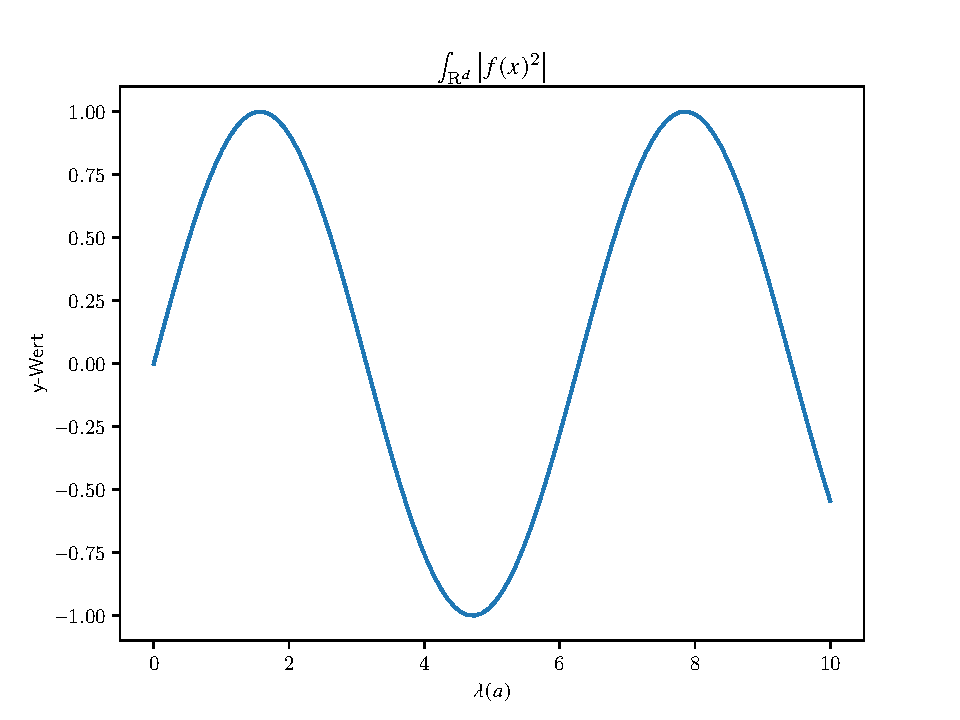
\includegraphics[width=0.5\textwidth]{figures/plot.pdf}
    \caption{Sine function}
    \label{fig:sinus}
\end{figure}




\newpage
\section{Basic Formalism}

Basic Definitions of schröfinger qe, light dyson series, and sotrong field s matrix


\newpage
\section{Strong Field Approximation}

clear defintition of the strong field approximation, and the assumptions that are made.



\newpage
\section{Strong Field Ionization}

Derivation of 

\begin{equation}
    \lim_{t \to \infty} \ket{\Psi(t)}  = -i \int d^3 p\, \ket{\mathbf{p}} \int_{-\infty}^{\infty} dt'\, e^{-\frac{i}{2}\int_{t'}^{\infty} [\mathbf{p}+\mathbf{A}(t')]^2 \, dt'} e^{i I_\mathrm{p} t'} \langle \mathbf{p} + \mathbf{A}(t') | \hat{\mathbf{d}} \cdot \mathbf{E}(t') | \Psi_0 \rangle
\end{equation}



\newpage
\section{Multiphoton Ionization}

Different types of Ionization, tunneling Ionization, multiphoton